\documentclass[a4paper11pt]{article}

\pagestyle{empty}


%%%%%%%%%%%%%%%%%%%%%%%%%%%%%%% Paquetes %%%%%%%%%%%%%%%%%%%%%%%%%%%%%%%%%%%

\usepackage[ansinew]{inputenc}
\usepackage[spanish]{babel}
\usepackage[mathcal]{euscript}
\usepackage{amsmath,amsfonts,amssymb,theorem,latexsym,mathrsfs, %hyperref,
            epsfig, multicol,anysize,graphicx,enumitem,mdwlist}
\usepackage{graphicx}  
\usepackage{ragged2e}  
\usepackage{float}        


%%%%%%%%%%%%%%%%%%%%%%%%%%%%%%%%%%%%%%%%%%%%%%%%%%%%%%%%%%%%%%%%%%%%%%%%%%%%


%%%%%%%%%%%%%%%%%%%%%%%%%%%%%%% M�rgenes %%%%%%%%%%%%%%%%%%%%%%%%%%%%%%%%%%%

\marginsize{2cm}{1cm}{1cm}{cm}

%\marginsize{izquierdo}{derecho}{arriba}{abajo}

%%%%%%%%%%%%%%%%%%%%%%%%%%%%%%%%%%%%%%%%%%%%%%%%%%%%%%%%%%%%%%%%%%%%%%%%%%%%


%%%%%%%%%%%%%%%%%%%%%%%%%%%%% Definiciones %%%%%%%%%%%%%%%%%%%%%%%%%%%%%%%%%

\def\r{\mathbb{R}}
\def\n{\mathbb{N}}
\def\q{\mathbb{Q}}
\def\c{\mathbb{C}}
\def\z{\mathbb{Z}}

\def\sen{\mathop{\mbox{\normalfont sen}}\nolimits}
\def\intt{\mathop{\mbox{\normalfont int}}\nolimits}
\def\diag{\mathop{\mbox{\normalfont diag}}\nolimits}
\def\arcsen{\mathop{\mbox{\normalfont arcsen}}\nolimits}
\def\ln{\mathop{\mbox{\normalfont ln}}\nolimits}
\def\tr{\mathop{\mbox{\normalfont tr}}\nolimits}

%%%%%%%%%%%%%%%%%%%%%%%%%%%%%%%%%%%%%%%%%%%%%%%%%%%%%%%%%%%%%%%%%%%%%%%%%%%%

\begin{document}

%%%%%%%%%%%%%%%%%%%%%%%%%%%% Encabezado %%%%%%%%%%%%%%%%%%%%%%%%%%%%%%%%%%%%

\begin{minipage}{0.12\linewidth}

\includegraphics[width=20mm]{escudo.jpg}
\end{minipage}
\begin{minipage}{0.78\linewidth}
\centerline{UNIVERSIDAD DE ANTIOQUIA}
\centerline{Facultad de Ciencias Exactas y Naturales}
\centerline{Instituto de Matem�ticas}
\centerline{Series de Tiempo I}
%\centerline{Taller $\#$ 1}
\end{minipage}

\vspace{3mm}

\leftline{Profesor: Duv�n Cata�o}


\vspace{8mm}


\begin{enumerate}

\item	 For a moving average process of the form 
$$x_t = w_{t-1} + 2w_t + w_{t+1},$$
where $w_t$ are independent with zero means and variance $\sigma_w^2$, determine the autocovariance and autocorrelation functions as a function of lag $h=s-t$ and plot the ACF as a function of $h.$ 

\bigskip

\item For an $MA(1)$, $x_t = w_t + \theta w_{t-1}$, show that $|\rho_x(1)|\leq1/2$.
 for any number $\theta$. For which values of $\theta$ does $\rho_x(1)$ attain its maximum and minimum?


\bigskip

\item A real-valued function $g(t),$ defined on the integers, is non-negative definite if and only if 

$$\sum_{i=1}^{n}\sum_{j=1}^{n}a_ig(t_i-t_j)a_j\geqslant0,$$

for all positive integers $n$ and for all vectors $a=(a_1, a_2, \ldots , a_n)'$ and $t=(t_1,t_2, \ldots ,t_n)'.$ For the matrix $G=\{g(t_i-t_j); i,j = 1,2, \ldots ,n\},$ this implies that $a'Ga\geqslant0$ for all vectors $a.$ 
  \begin{enumerate}
    \item[a.] Prove that $\gamma(h),$ the autocovariance function of a stationary process, is a non-negative definite function.\\
    
     \item[b.] Verify that the sample autocovariance $\hat{\gamma}(h),$ is a non-negative definite function.\\
\end{enumerate}

\bigskip

\item Identify the following models as ARMA$(p, q)$ models (watch out for parameter redundancy), and determine whether they are causal and/or invertible:
\begin{enumerate}
\item[a.] $x_t = 0.80x_{t-1} - 0.15x_{t-2} + w_t - 0.30w_{t-1}.$ 
\item[b.] $x_t =x_{t-1}-0.50x_{t-2}+w_t -w_{t-1}.$
\end{enumerate}
\bigskip

\item Suponga que los residuos $\hat{a}_t$ del modelo $(1-B)x_t=(1+0,6B)a_t,$ ajustado de una serie de 80 observaciones, proporcionan las siguientes autocorrelaciones:
\bigskip

\begin{table}[htdp]
\begin{center}\begin{tabular}{|c|c|c|c|c|c|c|c|c|c|c|}
\hline
$h$ & 1 & 2 & 3 & 4 & 5 & 6 & 7 & 8 & 9 & 10  \\
\hline
$\hat{\rho}_a(h)$ & 0.39 & 0.20 & 0.09 & 0,04 & 0,09 & -0.08 & -0.05 & 0.06 & 0.07 & -0.02\\
\hline
\end{tabular} 
\end{center}
\label{defaulttable}
\end{table} 

Analice la adecuaci{\'o}n del modelo ajustado y si existe alguna indicaci{\'o}n de falta de ajustamiento del modelo. Si esto ocurre, sugiera un modelo modificado.


\bigskip 
\newpage

\item Considere las siguientes ACF y PACF muestrales (estimadas) obtenidas a partir de una realizaci{\'o}n de tama{\~n}o $n=100$ de una serie de tiempo. 

\begin{table}[htdp]
\begin{center}\begin{tabular}{|c|c|c|c|c|c|c|c|c|c|c|}
\hline
$h$ & 1 & 2 & 3 & 4 & 5 & 6 & 7 & 8 & 9 & 10  \\
\hline
$\hat{\rho}(h)$ & -0.43 & 0.04 & 0.01 & -0.03 & 0.02 & 0.02 & 0.00 & -0.01 & -0.02 & 0.01 \\
\hline
$\hat{\phi}(h)$ & -0.43 & -0.33 & -0.25 & -0.18 & -0.13 & -0.08 & -0.04 & -0.04 & -0.02 & -0.01\\ 
\hline
\end{tabular} 
\end{center}
\label{defaulttable}
\end{table}

\begin{enumerate}
\item[a.] Obtenga los correlogramas.
\item[b.] ?`Qu{\'e} tipo de proceso parece ser el que genera los datos de la serie? Explique.
\item[c.] Escriba el modelo. Con excepci{\'o}n de la constante, cu{\'a}les ser{\'i}an unos estimadores preliminares para los par{\'a}metros del modelo?
\item[d.] Obtenga la forma dual de este modelo, usando los estimadores preliminares del punto c).
\end{enumerate}

\bigskip
\item Considere el modelo $x_t + \beta x_{t-1}=w_t.$
\begin{enumerate}
\item Obtenga una condici\'on de estacionaridad para $x_t.$
\item Encuentre la representaci\'on MA$(\infty).$
\item Obtenga la ACF de $x_t$ y graf\'iquela.
\end{enumerate}


\bigskip

\item Sea $y_t=a_{t}+ca_{t-1}+ca_{t-2}+\ldots+ca_1$, para $t>0,$ donde $c\in\mathbb{R}$ y $a_t\sim RB(0, \sigma_a^2).$
\begin{enumerate}
 \item[a.] Calcular la media y autocovarianza de $y_t$. ?`Es estacionaria? 
 \item[b.] Demostrar que la serie $z_t=(1-B)y_t$ es estacionaria.
\end{enumerate}

\end{enumerate}

\end{document}


% \begin{figure}[H]
%  \centering
%  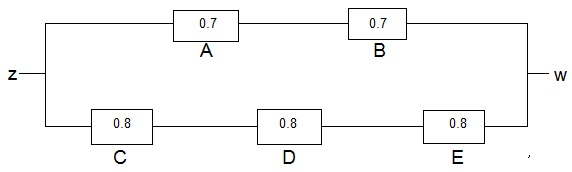
\includegraphics[width=.50\textwidth]{tab3}
% \end{figure}